\documentclass{standalone}
\usepackage{tikz}

\begin{document}
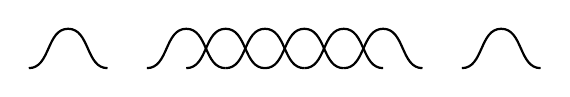
\begin{tikzpicture}
    % Draw the sequence of saddle moves and crossings
    % Start from left and move to right
    
    % First saddle (down-up)
    \draw[thick] (0,0) to[out=0,in=180] (0.5,0.5) to[out=0,in=180] (1,0);
    % Twist region with multiple crossings
    \foreach \x in {1.5,2,2.5,3,3.5,4} {
        \draw[thick] (\x,0) to[out=0,in=180] (\x+0.5,0.5) to[out=0,in=180] (\x+1,0);
    }
    % Last saddle (up-down)
    \draw[thick] (5.5,0) to[out=0,in=180] (6,0.5) to[out=0,in=180] (6.5,0);
    
\end{tikzpicture}
\end{document}